\chapter{Records}

Given a permutation $A = A_1 A_2 A_3 \ldots A_n$, $A_i$ is a
\emph{record} if it is a maximum of all preceding elements.

\section{Harmonic Number}

What is the expected number of records in $A$?

Let $I_i$ be an indicator random variable with value 1 only if $A_i$
is a record.  We know that there are $(i-1)!$ many permutations where
$A_i$ is maximum, and $i!$ total permutations, which gives 

\begin{displaymath}
  E(I_i) = Pr(I_i = 1) = \frac{(i-1)!}{i!} = \frac{(i-1)!}{i (i-1)!} = \frac{1}{i}
\end{displaymath}

Let the expected number of records in $A$ be $X$.

\begin{align*}
  %
  E(X)
  &= E \left( \sum_{i=1}^{n} I_i \right) \\
  &= \sum_{i=1}^{n} E(I_i) \\
  &= \sum_{i=1}^{n} \frac{1}{i} \\
  %
\end{align*}

This sum is the $i$th \emph{harmonic number}, denoted $H_i$.

We know that $H_n = \BigTheta{\log n}$.  In fact, $ \left| H_n - \log
  n \right| \le 1$.  See Figure \ref{fig:HarmonicNumbers}.

Historical note: the theory of records was first applied to the
analysis of data structures by Luc Devroye in 1988\cite{Devroye:1988}.
Luc Devroye noted that the number of elements along the search path in
a binary search tree is the number of max records less than the search
element plus the number of min records greater than the search
element.


\begin{figure*}
  \label{fig:HarmonicNumbers}
  \centering
  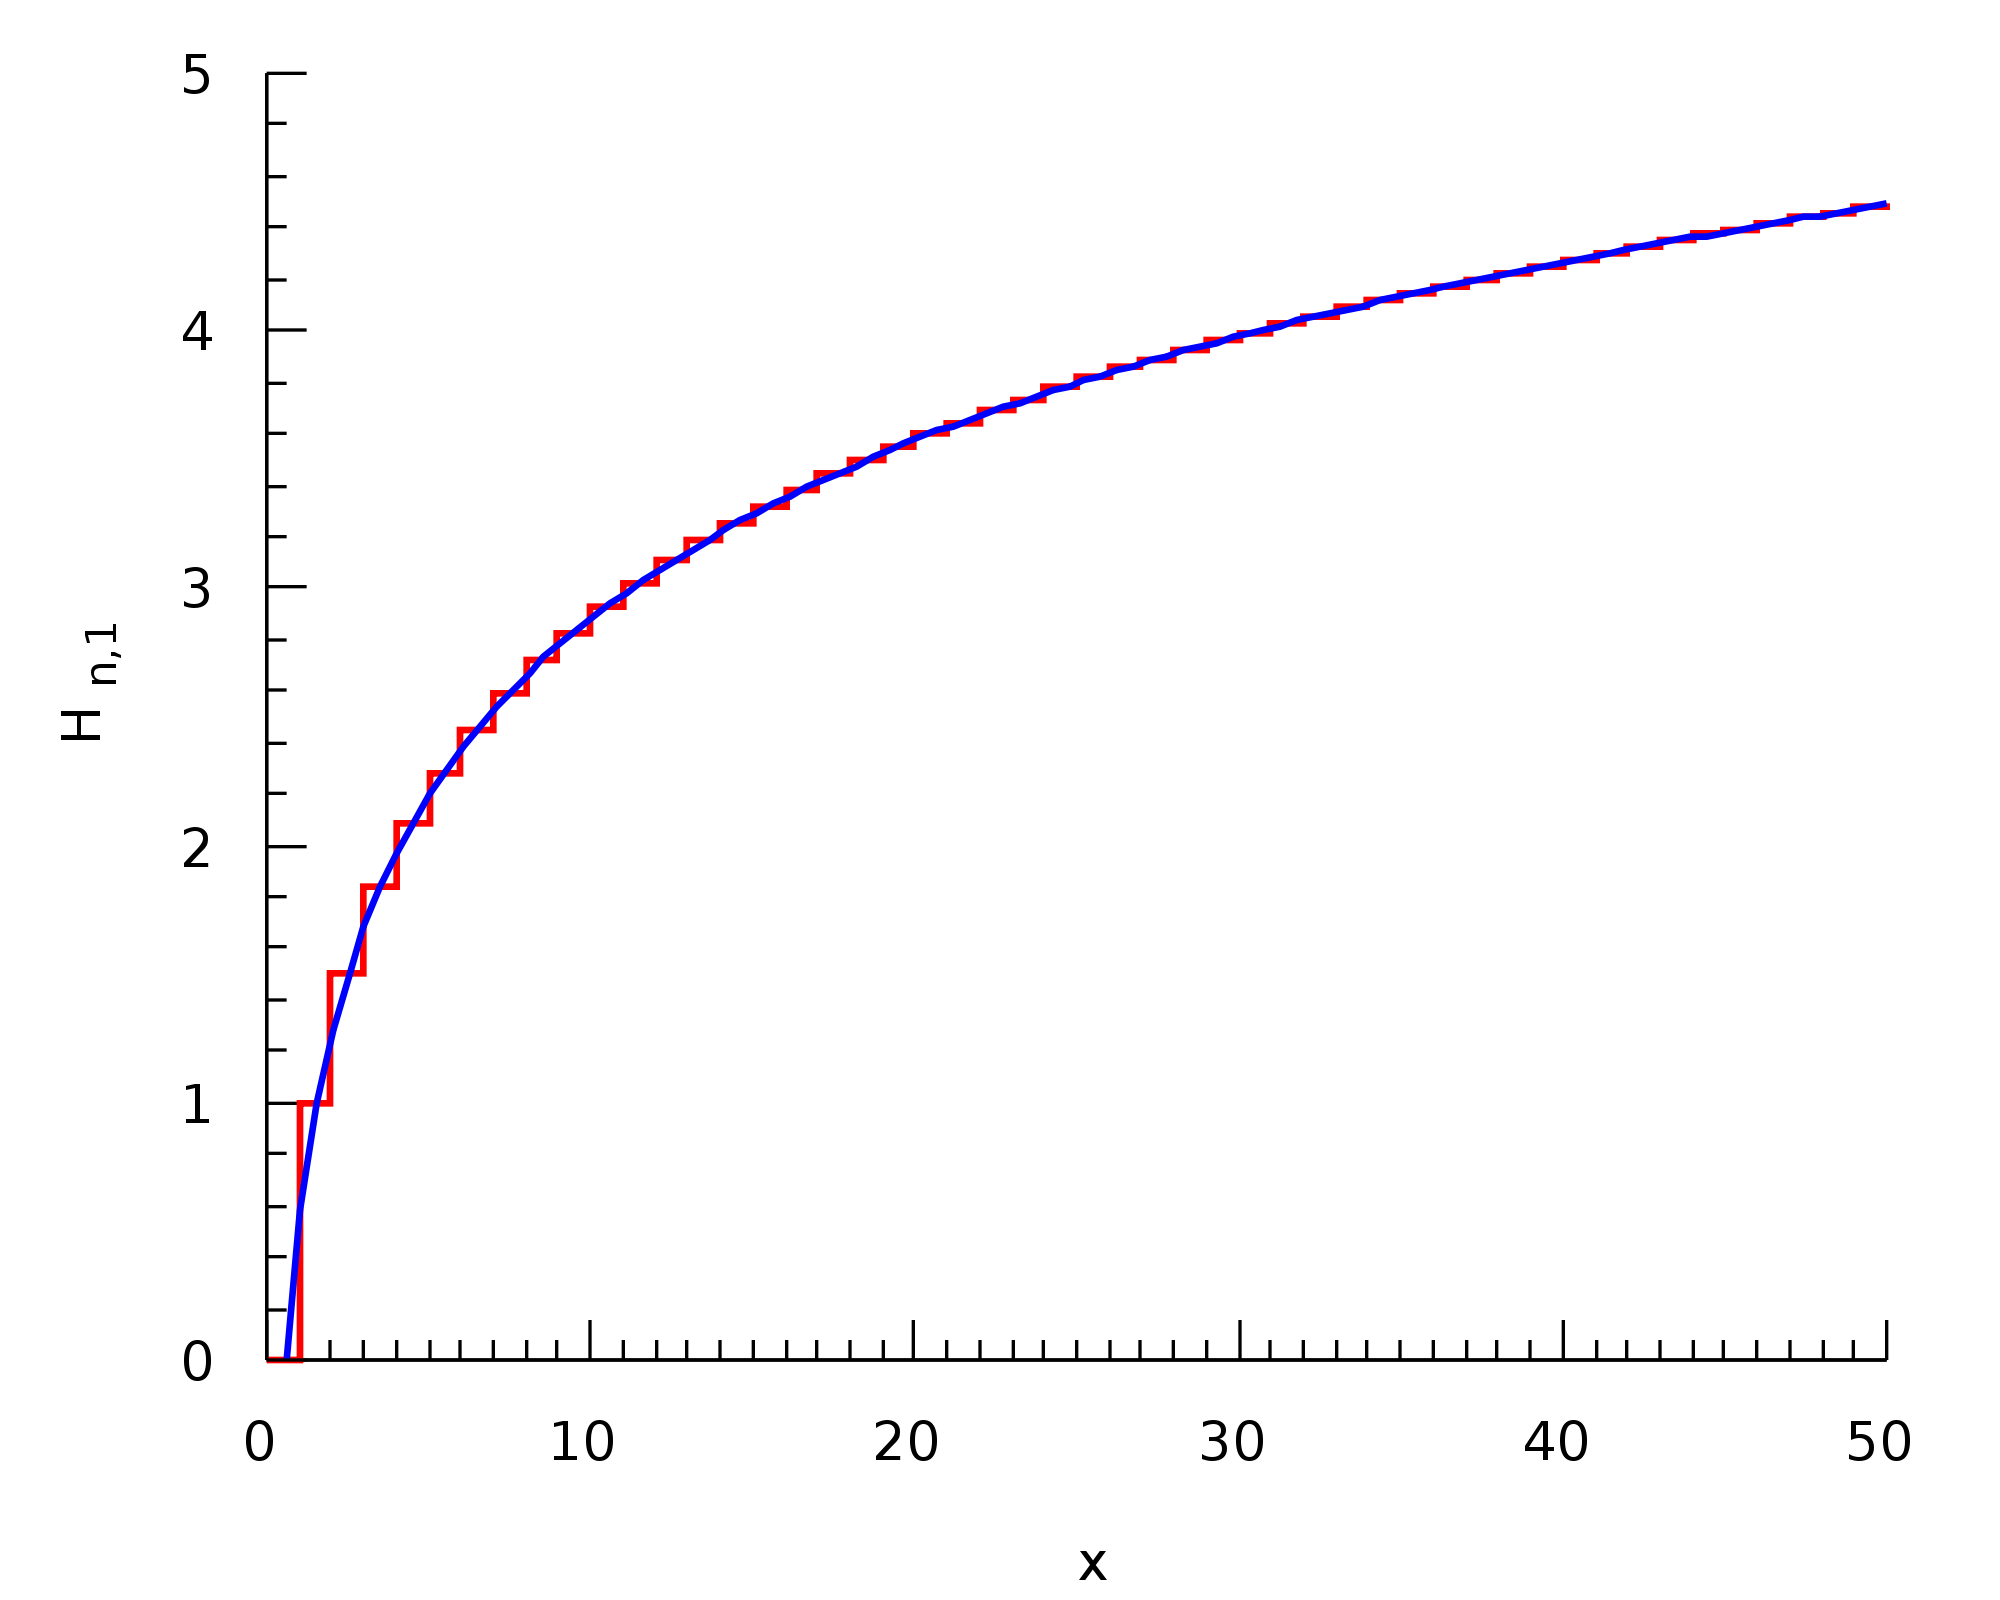
\includegraphics[scale=0.25]{HarmonicNumbers}
  \caption{A chart of the harmonic numbers compared to $\log n$}  
\end{figure*}